%追加すべき事項
% - "音楽の表現"における音声処理の補強
% - "音楽の表現"の式(理解が必要)
% - "音楽の表現"の具体例(論文,既存研究)
% - "音楽の表現"の図
% - "音楽の表現"の単語の説明
\chapter{背景:音楽}

本章では、本論文での音の定義を行った後に、音楽の特徴量抽出の方法を紹介する。

\section{音の定義}

音とは、弾性体中を伝播する弾性波により起こされる音波の信号~(音響信号)~が聴覚により感じられるもののことである。また、音は騒音と楽音の大きく二つに分けることができる。騒音とは不規則な振動の音波による音のことであり、楽音とは周期性のある音波による音のことである。そして、本論文では楽音を音と定義するが、楽音は長さ、大きさ、高さ、音色の四要素を持つ。ここで、\prettyref{fig:gakuon1}はある音波の図であり、\prettyref{fig:gakuon2}はその音波の適当な部分の拡大図である。

\subsection{音の長さ}

音の長さは音波の時間長として定義する~(\prettyref{fig:gakuon1})~。また、音の長さは楽譜上での時間の長さ~(音価)~として一般には定義される。

\subsection{音の大きさ}

音の大きさは音波の振幅により決まる~(\prettyref{fig:gakuon1})~。また、人間は振幅の大きい音ほど大きく知覚する。

\begin{figure}[b]
\centering
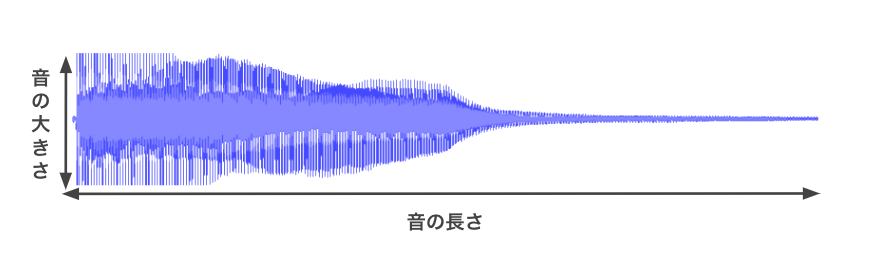
\includegraphics[width=\columnwidth]{figure/gakuon1.png}
\caption{音波}
\label{fig:gakuon1}
\end{figure}

%ここで改ページ
\clearpage

\subsection{音の高さ}

音の高さは音波の周波数により決まる。直感的には、音波の周期構造の長さにより決まる~(\prettyref{fig:gakuon2})~。また、人間は周波数の高い音ほど高く知覚する。

\subsubsection{単音と重音}

ある楽器である高さの一音を鳴らした時に出力される音を単音と呼ぶ。また、ほとんどの単音は複数の周波数の音波の合成波であり、最も低い周波数成分の音~(基音)~の高さを音の高さとして人間は知覚する。そして、この単音の音を重ね合わせた音のことを重音と呼ぶ。

\subsubsection{音階表記}

本論文では、西洋音楽で用いられる12音階の表記を音の高さを表すために使用する。この表記では、$C,C^{\sharp},D,D^{\sharp},E,F,F^{\sharp},G,G^{\sharp},A,A^{\sharp},B$の12段階の音の高さの集合をオクターブとして定める。そして、それぞれのオクターブに番号を振り、440~Hzの音をA4と定めることで音の高さの絶対的な表記を可能にしている。また、この表記で表す音を半音と呼ぶが、半音より細かい音~(微分音)~を表すことはできない。ただし、本論文では半音のみを音の高さとして扱う。

\subsection{音の音色}

音の長さと大きさと高さが同じであっても異なった音として人間には知覚されることがある。この違いを音色と呼び、別の楽器は異なった音色を持つ。直感的には、音色は音波の周期構造の形により決まる~(\prettyref{fig:gakuon2})~。また、この周期構造の違いは基音より高い音~(上音)~の音波の組み合わせの違いに起因する。

\begin{figure}[b]
\centering
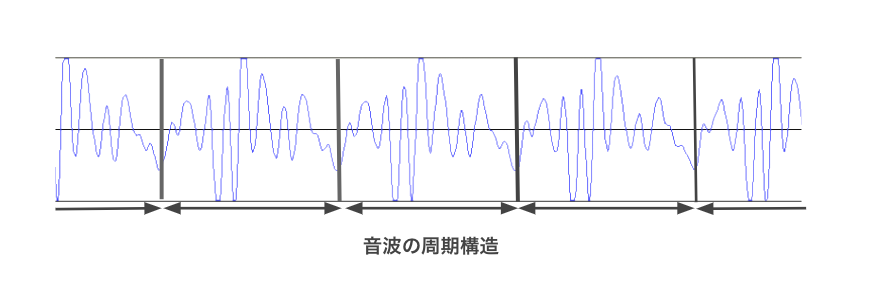
\includegraphics[width=\columnwidth]{figure/gakuon2.png}
\caption{音波の拡大図}
\label{fig:gakuon2}
\end{figure}

%ここで改ページ(したい)
\clearpage

\section{音の表現}
\label{sec:preprocess}

音をニューラルネットワークで扱うためには、楽音としての特徴を学習するための適切な表現を得る必要がある。また、本節は~\cite{musictutorial}を参考に作成し、本節の図は~\cite{musictutorial}のFigure~4を利用している。

\subsection{音響信号}

アナログ信号の音響信号をデジタル信号へと変換した一次元データが基本的な表現である~(\prettyref{fig:audio_signal})~。また、デジタル信号への変換の際には標本化~(サンプリング)~と量子化が必要である。まず、サンプリングはアナログ信号を一定の時間を空けて離散的に測定を行うことであり、1秒あたりのサンプリング回数をサンプリング周波数と呼ぶ。そして、量子化は信号の大きさを離散的に近似して表現することであり、信号の大きさの細かさを表現するビット数を量子化ビット数と呼ぶ。

%どの点が音響信号で良いから〇〇では用いられた
音響信号は音の素朴な表現であるため、〇〇などの研究では△△という長所を利用して音響信号を直接利用している。

\begin{figure}[b]
\centering
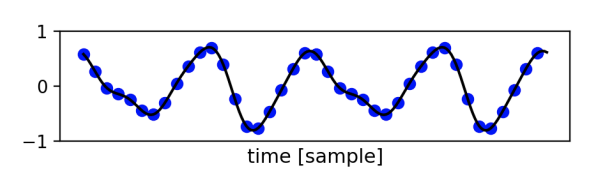
\includegraphics[width=0.8\columnwidth]{figure/audio_signal.png}
\caption{音響信号}
\label{fig:audio_signal}
\end{figure}

\subsection{二次元での表現}

音響信号は素朴な表現の一次元データであるが、ニューラルネットワークが楽音としての特徴を学習するには多くのデータが必要になると考えられる。、次節以降で紹介するような二次元データへと変換して扱うことが一般的である。また、中心周波数を利用したバンドパスにより音響信号を周波数成分ごとに分解する変換を行うことが多い。これにより、時間-周波数表現へと変換できるため、信号が明確化されより効果的な表現として扱うことができる。

そして、二次元の場合は画像のニューラルネットワークを流用できることも多いが、この場合は主に二つの相違点に注意が必要である。一つ目は、局所的な相互関係についてである。画像では近くのピクセル同士の色合いや強度が似ているが、時間-周波数表現では周波数方向での局所的な相互関係が弱い。二つ目は、スケール不変性についてである。画像ではスケールを変化させても特徴は不変であることが多いが、時間-周波数表現ではスケールを変化させることで特徴は変化する。

%ここで改ページ
\clearpage

\subsection{STFT}

STFT~(Short~Time~Fourier~Transform)~は時間-周波数表現を生成する基本的な手法であり、中間周波数を利用した線形間隔のバンドパスフィルターを用いて周波数成分を分解する。また、横軸を時間で縦軸を周波数とした画像をSTFTにより生成することができ、これをスペクトログラムと呼ぶ。ここで、STFTの具体的な計算方法については〇〇に詳しい。%勉強する

しかし、人間の聴覚系の周波数分解能は線形ではないかつ楽音の解析のために作成されたわけではないため、STFTのバンドパスは楽音の解析に適しているとは言えない。したがって、STFTはニューラルネットワークで扱う表現の作成において人気のある手法ではない。ただし、STFTは音源分離などに用いられることがある。%研究例を挙げる

\subsection{メルスペクトログラム}

メルスペクトログラムはメル尺度~\cite{melscale}を用いてスペクトログラムにおいて周波数方向の圧縮を行ったものである。また、メル尺度は人間の感じる音の高さの差と差が等しくなるように調整した尺度であり、~\cite{mel}では周波数を$f$として\prettyref{eq:mel}のように定式化される。

\begin{align}
    \label{eq:mel}
    mel(f)=1127.01048\log{(\frac{f}{700}+1)}
\end{align}

メル尺度は人間の聴覚系に合わせた尺度であるため、スペクトログラムよりも楽音の解析に適している。また、経験的にもメルスペクトログラムは楽音のタスクに適していることが言える。%研究例

\begin{figure}[b]
\centering
\begin{minipage}{0.48\columnwidth}
\centering
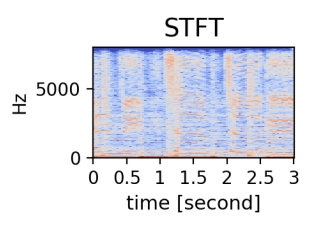
\includegraphics[width=\columnwidth]{figure/stft.png}
\caption{STFT}
\label{fig:STFT}
\end{minipage}
\begin{minipage}{0.48\columnwidth}
\centering
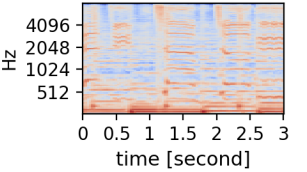
\includegraphics[width=\columnwidth]{figure/mel.png}
\caption{メルスペクトログラム}
\label{fig:mel}
\end{minipage}
\end{figure}

%ここで改ページ
\clearpage

\subsection{CQT}

CQT~(Constant~Q~Transform)~は対数振幅の中心周波数を使用した二次元の表現である。CQTは対数振幅を用いており、音の高さの分布に近い。したがって、基音を正確に識別する際に用いられ、和音の識別や書き換えに使うことができる。

また、計算量としてはSTFTやメルスペクトログラムより重い。そして、単純な対数振幅のスペクトログラムが有効な例もある。

\subsection{クロマグラム}

与えられた音の高さの集合におけるエネルギー分布のこと。多くの場合は西洋音楽の12音階をその集合とする。つまり、クロマグラムは周波数方向に畳み込んだCQTと見なすことができる。また、クロマグラムは他の表現方法よりも処理が進んだものなので、それ自身を特徴量として用いることができる。

\begin{figure}[b]
\centering
\begin{minipage}{0.48\columnwidth}
\centering
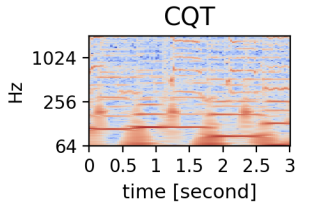
\includegraphics[width=\columnwidth]{figure/cqt.png}
\caption{CQT}
\label{fig:cqt}
\end{minipage}
\begin{minipage}{0.48\columnwidth}
\centering
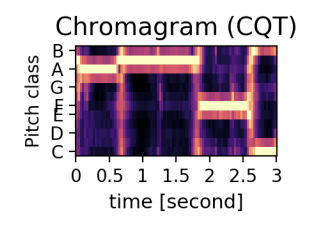
\includegraphics[width=\columnwidth]{figure/choroma.png}
\caption{クロマグラム}
\label{fig:chroma}
\end{minipage}
\end{figure}
    
%ここで改行
\clearpage


%ここを提案モデルにもいれよう

\section{音楽の特徴}

一般には音楽で特定の音色への変換を行うことは難しいが、本研究では三つの要素に分解することで単音での音色の変換を音楽へと適用することが可能であると考えた。

\subsection{楽器の重ね合わせ}
    
音楽はそれぞれの楽器から出力される音の重ね合わせになっている。楽器ごとに音色は異なるため、音色変換を行うには楽器ごとの音波に分解すること~(音源分離)~が必要であると考えられる。なお、楽曲の作成時に楽器ごとに分離したデータ~(パラデータ)~として保存することが一般的であるため、パラデータの公開が一般的になれば音源分離の必要はなくなる。

\subsection{音の重ね合わせ}

ある音が重音である場合はそれぞれの単音について音色変換を行う必要がある。本研究では、データセットとして単音のみを使用するが、重音もデータセットに加えることで音色変換が可能であると考えられる。また、この際にデータセットが膨大な量になる可能性があり、追加するデータセットの工夫が必要である。

\subsection{音の繋ぎ方}

楽器ごとの音波に分解可能で重音も表現可能である時、時間方向の音の繋ぎ方を工夫する必要がある。また、単音の変換を一定の単位時間で行うことで、音楽もその単位時間で分割して変換することで可能であると考えられる。ただし、単位時間の定め方により性能が変わると考えられるので、単位時間は慎重に定める必要がある。

%ここで改ページ

